\documentclass{article}

\usepackage{amsmath,graphicx,parskip}
\usepackage{epstopdf}
\usepackage{fancyhdr}
\usepackage[english]{babel}
\usepackage{verbatim}
\usepackage[top=3cm,bottom=3cm]{geometry}
\pagestyle{fancy}
\lhead{Samuel Cole Huberman}
\chead{MIE1011}
\rhead{999157923}

\begin{document}

\section*{Chapter 2 Question 2}

\subsection*{Part A}
From the energy and entropy postulates
\begin{align*}
0&\ge \Delta U^C-T^R\Delta S^C+P^R \Delta S^C-\mu^R \Delta N^C
\end{align*}
Expanding and noting conservation of molecules and $P^R=P^S$
\begin{align*}
0&\ge \Delta (U^S+U^S+U^{LS}+U^R)-T^R\Delta (S^L+S^S+S^{LS}+S^R)+P^R \Delta (S^L+S^S)\\
&\ge \Delta(U^S+T^RS^S+P^RS^S+\Delta(U^L+T^RS^L)+\Delta(U^{LS}+T^RS^{LS}) +P^S \Delta S^L\\
&\ge \Delta(G^S+F^L+F^{LS}+P^S S^L)
\end{align*}
Defining
\begin{align*}
D=\Delta(G^S+F^L+F^{LS}+P^S S^L)
\end{align*}
Any arbitrary change would increase B, so at equilibrium, B must be at a minimum.
\begin{align*}
G^S&=N^S_1\mu^S_1+N^S_2\mu^S_2\\
F^L&=-P^LS^L+N^L_2\mu^L_S\\
F^L&=A^{LS}\gamma^{LS}+N^{LS}_2\mu^{LS}_2+N^{LS}_1\mu^{LS}_1\\
\end{align*}

\subsection*{Part B}
Taking virtual displacements of $B$
\begin{align*}
dB&=dG^S+dF^L+dF^{LS}+P^R dS^L\\
&=\sum_i^2\mu^S_i dN^S_i+(-P^LdS^L +\mu ^L_2 dN^L_2)+(\gamma^{LS}dA^{LS} +\sum_i^2\mu ^{LS}_i dN^{LS}_i)+P^{S}dS^L
\end{align*}
such that the constraints require
\begin{align*}
dN^L_2&=-N^S_2-N^{LS}_2\\
N^S_1&=-N^{LS}_1\\
dS^L&=4 \pi R^2 dR\\
dA^{LS}&= 8 \pi R dR
\end{align*}
which yields
\begin{align*}
dB&=(\mu^L_2-\mu^S_2)dN^S+\sum_i^2(\mu^{LS}_i-\mu^S_i)dN^{LS}+(-4\pi R^2P^L+4\pi R^2P^S+8\pi\gamma^{LS}R)dR
\end{align*}
Thus the constraints for equilibrium are
\begin{align*}
\mu^S_2&=\mu^L_2=\mu^{LS}_2\\
P^L &=P^S +\frac{2\gamma^{LS}}{R_\delta}
\end{align*}

\subsection*{Part C}
Using the Gibbs-Duhem relation
\begin{align*}
v^L=\frac{\partial \mu_2^L(T,P^L)}{\partial P^L}_T=v(T,P^R)\exp[\kappa_T(P^R-P^L)]
\end{align*}
if $\kappa=\kappa(T)$, then we can write chemical potential of component 2 in the liquid phase
\begin{align*}
\mu_2^L(T,P^L)=\frac{v(T,P^R)}{\kappa_T}\exp[\kappa_T(P^R-P^L)]+f(T)
\end{align*}
The chemical potential of component 2 in the weak solution
\begin{align*}
\mu_2^L(T,P^S,N_1^S,N_2^S)=\mu_2^0(T,P^R)+RT\ln\frac{N_2^S}{N^2_{2sat}(T,P^S)}
\end{align*}

\subsection*{Part D}
Setting the component 2 chemical potentials equal
\begin{align*}
\mu_2^L(T,P^L)&=\mu_2^L(T,P^S,N_1^S,N_2^S)\\
\end{align*}
For $\kappa_T(P^R-P^L)<<1$, we have
\begin{align*}
v_{f2}(P^L-P^R)&=RT\ln\frac{N_2^S}{N^2_{2sat}(T,P^S)}\\
v_{f2}\frac{2\gamma^{LS}}{R_\delta}&=RT\ln\frac{N_2^SKh(T)}{N_1P^R}
\end{align*}
Rearranging
\begin{align*}
{R_\delta}&=\frac{2\gamma^{LS}}{\frac{RT}{v_{f2}}\ln\frac{N_2^SKh(T)}{N_1P^R}}
\end{align*}
Noting that $V^L=v_{f2}N^L_2=\frac{4\pi R^3}{3}$
\begin{align*}
{R_\delta}&=\frac{2\gamma^{LS}}{\frac{RT}{v_{f2}}\ln\frac{(N_2-\frac{4\pi R^3}{3v_{f2}})Kh(T)}{N_1P^R}}
\end{align*}

\subsection*{Part E}
\begin{figure}%[H]
\begin{center}
\scalebox{1}{ 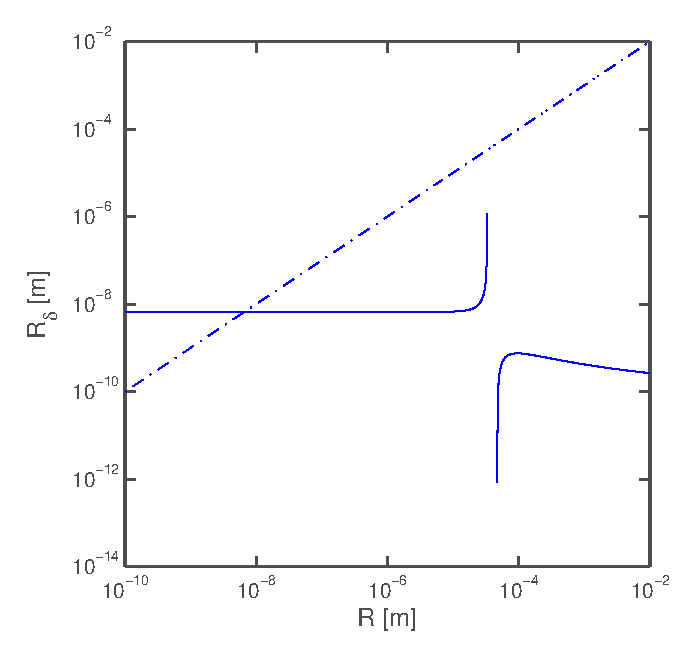
\includegraphics{plot.eps}}
\renewcommand{\figure}{Fig.}
\caption{R vs R_\delta}
\end{center}
\end{figure}
The points of intersection with the direct linear plot of $R$ are
6.61e-9 and 3.31e-5 [m].
\\
\\
\subsection*{Part F}
For a single phase weak solution
\begin{align*}
D_0=\mu^S_1N^S_1+\mu^S_2-N^S_2
\end{align*}
\begin{align*}
D-D_0=(-P^L+P^R)V^L+\sum^2_iN^L(\mu^L_i-\mu^S_i)+\sum^2_iN^{LS}(\mu^{LS}_i-\mu^S_i)+\gamma^{LV}A^{LV}
\end{align*}
Since the chemical potentials are equal
\begin{align*}
D-D_0=4\pi \gamma^{LV}(R^2-\frac{2R^3}{3R_\delta})
\end{align*}

\begin{figure}%[H]
\begin{center}
\scalebox{1}{ 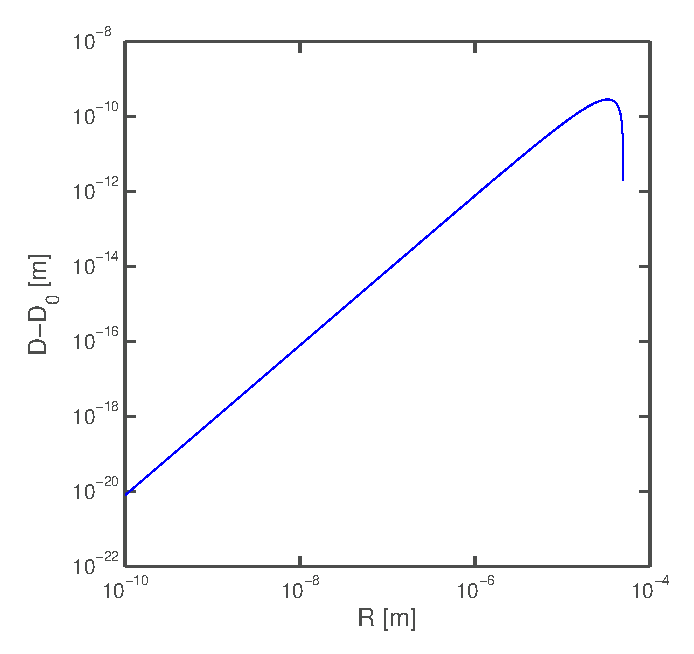
\includegraphics{plot2.eps}}
\renewcommand{\figure}{Fig.}
\caption{For $R_\delta$=3.31e-5}
\end{center}
\end{figure}

\begin{figure}%[H]
\begin{center}
\scalebox{1}{ \includegraphics{plot3.eps}}
\renewcommand{\figure}{Fig.}
\caption{For $R_\delta$=6.6e-9 (Not physical!)}
\end{center}
\end{figure}

\end{document}
